%%%%%%%%%%%%%%%%%%%%%%%%%%%%%%%%%%%%%%%%%
% University/School Laboratory Report
% LaTeX Template
% Version 3.0 (4/2/13)
%
% This template has been downloaded from:
% http://www.LaTeXTemplates.com
%
% Original author:
% Linux and Unix Users Group at Virginia Tech Wiki 
% (https://vtluug.org/wiki/Example_LaTeX_chem_lab_report)
%
% License:
% CC BY-NC-SA 3.0 (http://creativecommons.org/licenses/by-nc-sa/3.0/)
%
%%%%%%%%%%%%%%%%%%%%%%%%%%%%%%%%%%%%%%%%%

%----------------------------------------------------------------------------------------
%	PACKAGES AND DOCUMENT CONFIGURATIONS
%----------------------------------------------------------------------------------------

\documentclass{article}

\usepackage[version=3]{mhchem} % Package for chemical equation typesetting
\usepackage{siunitx} % Provides the \SI{}{} command for typesetting SI units

\usepackage{graphicx}
\usepackage{caption}
\usepackage{subcaption}
\usepackage{cancel}

\usepackage{float}

\usepackage[T1]{fontenc} % allow small bold caps

\usepackage{listings}
\usepackage{color}

\definecolor{dkgreen}{rgb}{0,0.6,0}
\definecolor{gray}{rgb}{0.5,0.5,0.5}
\definecolor{mauve}{rgb}{0.58,0,0.82}

\lstset{frame=tb,
  language=Matlab,
  aboveskip=2mm,
  belowskip=2mm,
  showstringspaces=false,
  columns=flexible,
  basicstyle={\small\ttfamily},
  numbers=none,
  numberstyle=\tiny\color{gray},
  keywordstyle=\color{blue},
  commentstyle=\color{dkgreen},
  stringstyle=\color{mauve},
  breaklines=true,
  breakatwhitespace=true
  tabsize=2
}

\setlength\parindent{0pt} % Removes all indentation from paragraphs

\renewcommand{\labelenumi}{\alph{enumi}.} % Make numbering in the enumerate environment by letter rather than number (e.g. section 6)

\usepackage[margin=1in]{geometry}

\usepackage{amssymb}


%\usepackage{times} % Uncomment to use the Times New Roman font

%----------------------------------------------------------------------------------------
%	Title
%----------------------------------------------------------------------------------------

\begin{document}
\pagenumbering{gobble}

\title{6.s02: EECS II - From A Medical Perspective}
\author{
  Ryan Lacey <rlacey@mit.edu>\\
  \footnotesize \texttt{Collaborator(s): Jorge Perez}
}
        
\maketitle
        


\begin{enumerate}
\item[1.]
	\begin{enumerate}
	\item[(a)]
		Frequency spectrum of glucose and ECG signals.
	
	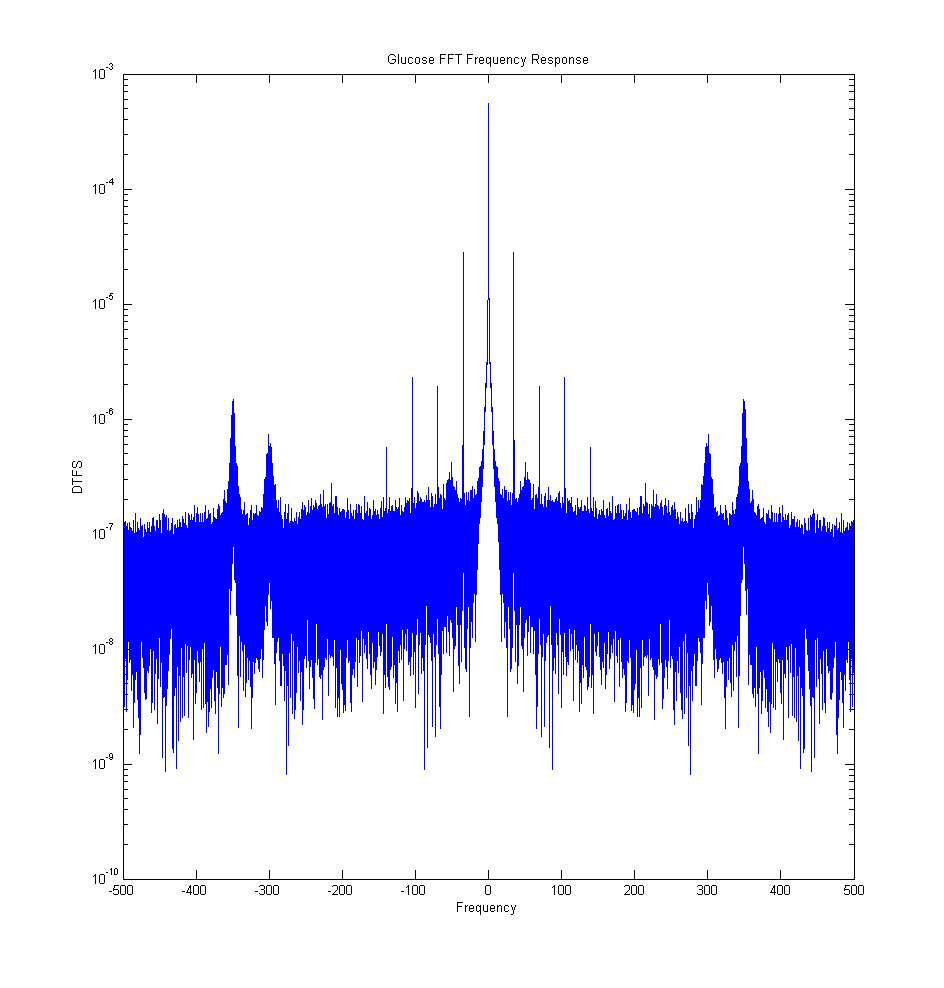
\includegraphics[width=\linewidth/2]{../images/P1_GlucoseFFT} \includegraphics[width=\linewidth/2]{../images/P1_ECGFFT}\\
 
 \bigskip
 
\begin{lstlisting}   
N = length(xg0);

xg0fftUnshifted = fft(xg0)/N;
xe0fftUnshifted = fft(xe0)/N;

xg0fft = fftshift(xg0fftUnshifted);
xe0fft = fftshift(xe0fftUnshifted);

f = linspace(-500, 500*(1-1/N), N);

semilogy(f, abs(xg0fft));
xlabel('Frequency');
ylabel('DTFS');
title('Glucose FFT Frequency Response');

semilogy(f, abs(xe0fft));
xlabel('Frequency');
ylabel('DTFS');
title('ECG FFT Frequency Response');
\end{lstlisting}

\newpage

	\item[(b)]
	Energy spectral density of glucose and ECG signals.\\
	
	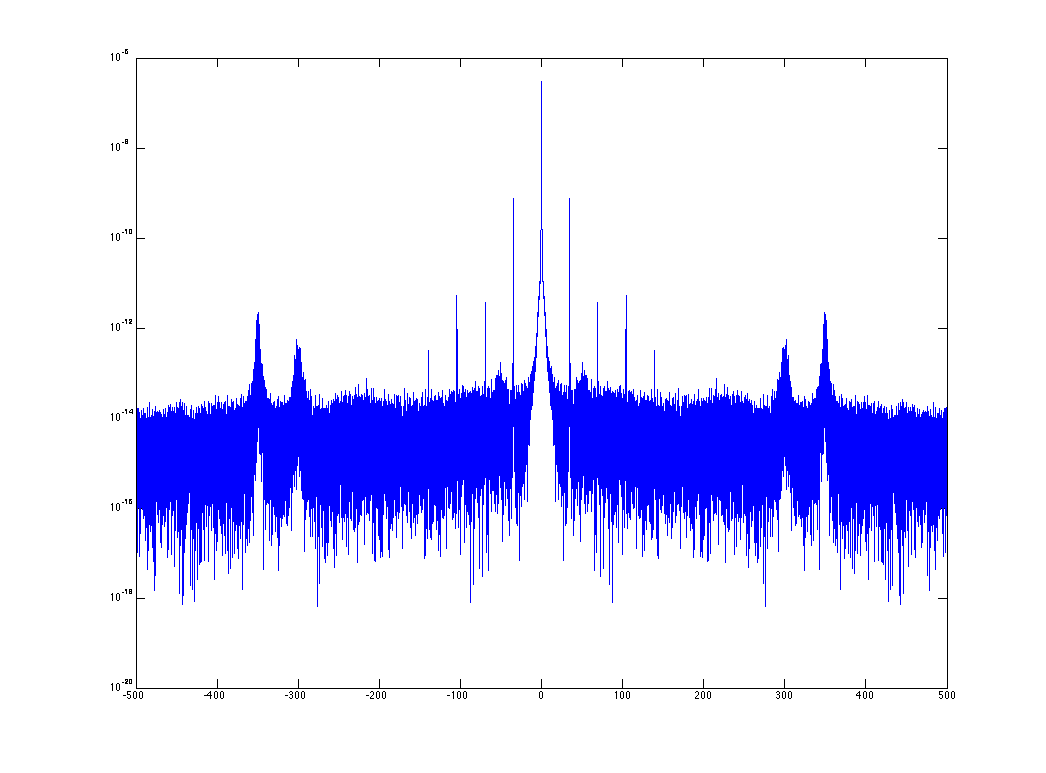
\includegraphics[width=\linewidth/2]{../images/P1_EDGlucose} 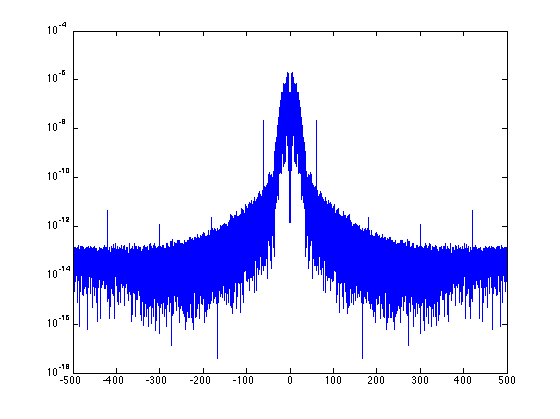
\includegraphics[width=\linewidth/2]{../images/P1_EDECG}\\

\bigskip

\begin{lstlisting}
% Using variables defined in (1a)
xg0s = abs(xg0fftUnshifted).^2;
xg0sfft = fftshift(xg0s);
semilogy(f, xg0sfft);

xe0s = abs(xe0fftUnshifted).^2;
xe0sfft = fftshift(xe0s);
semilogy(f, xe0sfft);
\end{lstlisting}

\bigskip

	\item[(c)] $\:$ \\
\begin{tabular}{l*{4}{c}r}
Glucose        &   1    &   5      &  100     &  500       \\
\hline
$E_T$          & 0.0850   & 0.0850   &  0.0850  &  0.0850  \\
$E(f_1,f_2)$   & 2.0e-04  & 8.1e-05  & 1.77e-05 & 1.0e-11  \\
Ratio          & 0.0024   & 9.6e-04  & 2.09e-04 & 1.2e-10  \\
\end{tabular}

\bigskip

\begin{tabular}{l*{4}{c}r}
ECG            &   1    &   5      &  100     &  500       \\
\hline
$E_T$          & 21.622   & 21.622   &  21.622  &  21.622  \\
$E(f_1,f_2)$   & 10.810   & 8.4107   & 1.7e-04  & 2.6e-09  \\
Ratio          & 0.5000   & 0.3890   & 7.9e-06  & 1.2e-10  \\
\end{tabular}

\bigskip

\begin{lstlisting}
% Using variables defined in (1a) and (1b)
f1 = 500;
f2 = 500;

k1 = N*f1 / 1000;
k2 = N*f2 / 1000;

EtG = N * sum(xg0s);
EfG = N * sum(xg0sfft(floor(k1+(N-1)/2):floor(k2+(N-1)/2)));
GlucoseRatio = EfG / EtG;

EtE = N * sum(xe0s);
EfE = N * sum(xe0sfft(floor(k1+(N-1)/2):floor(k2+(N-1)/2)));
ECGRatio = EfE / EtE;
\end{lstlisting}

\bigskip

	\item[(d)]
	placeholder

	\end{enumerate}

\newpage

\item[2.]
	Fourier coefficients of notch filter\\
	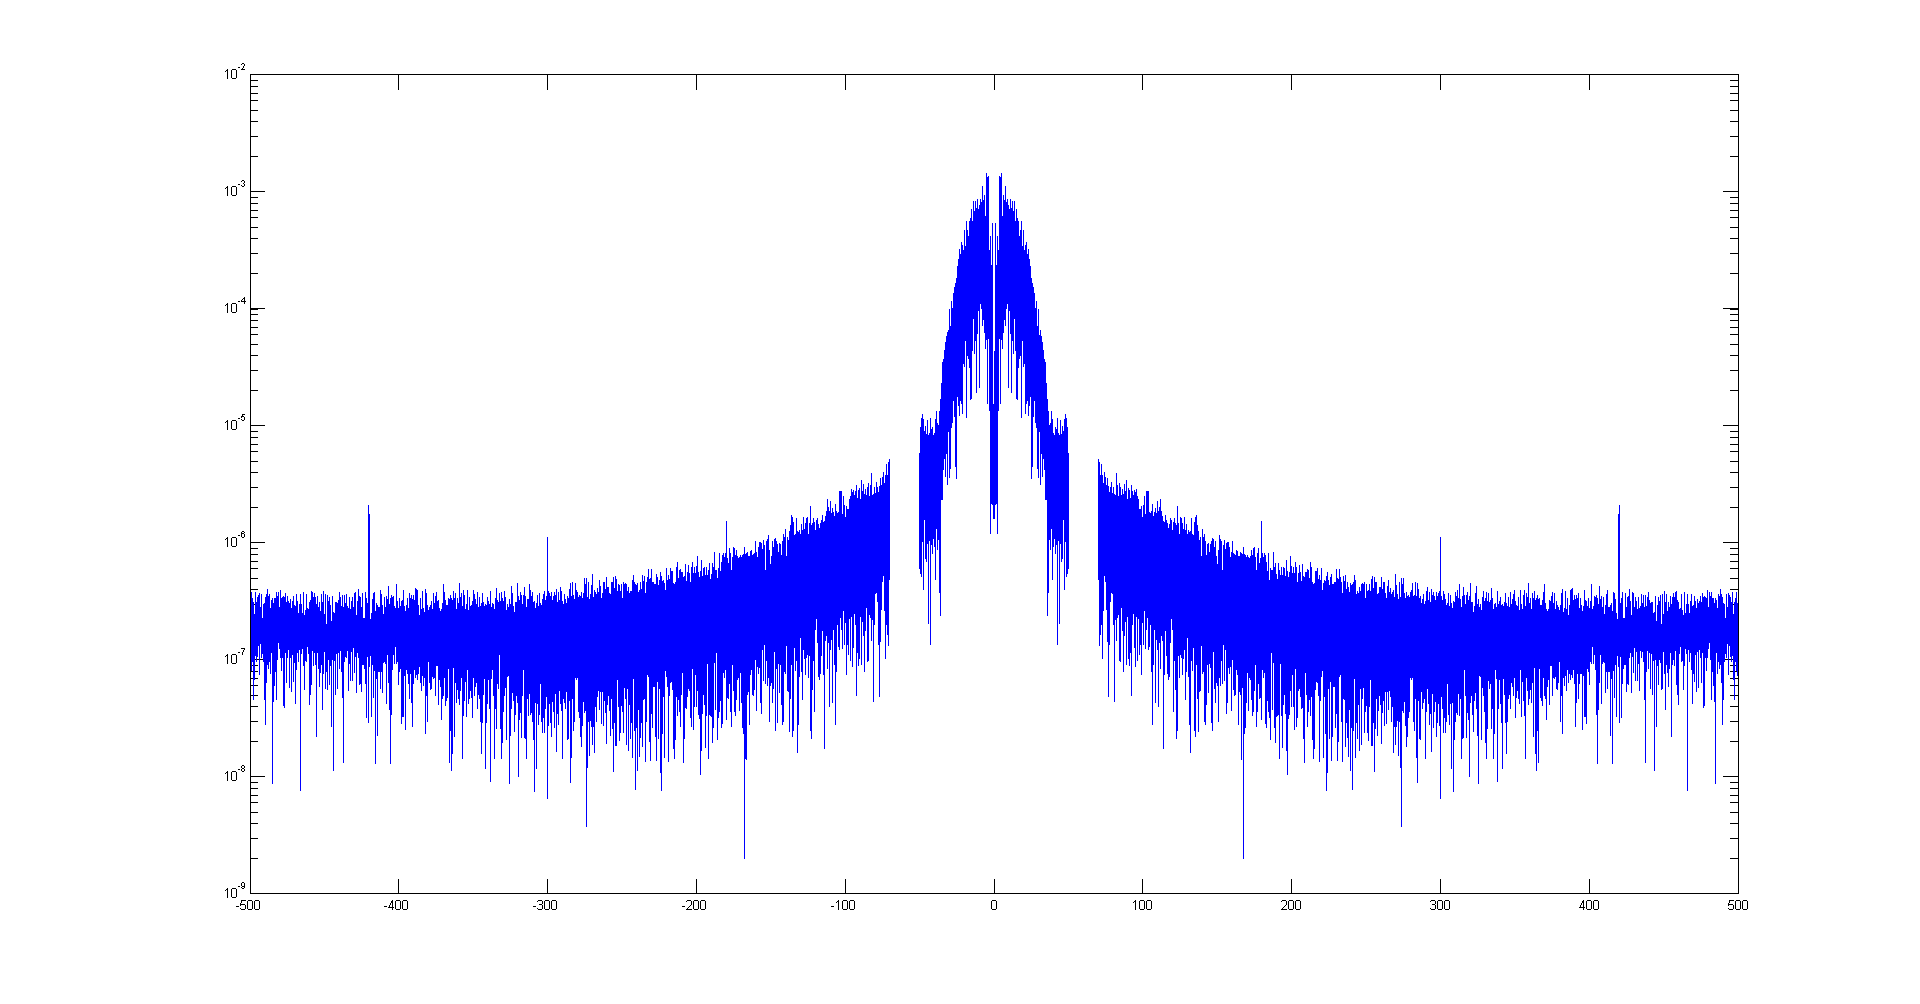
\includegraphics[scale=0.25]{../images/P2_FilteredFourierCoefficients} \\
	
	Filtered ECG signal\\
	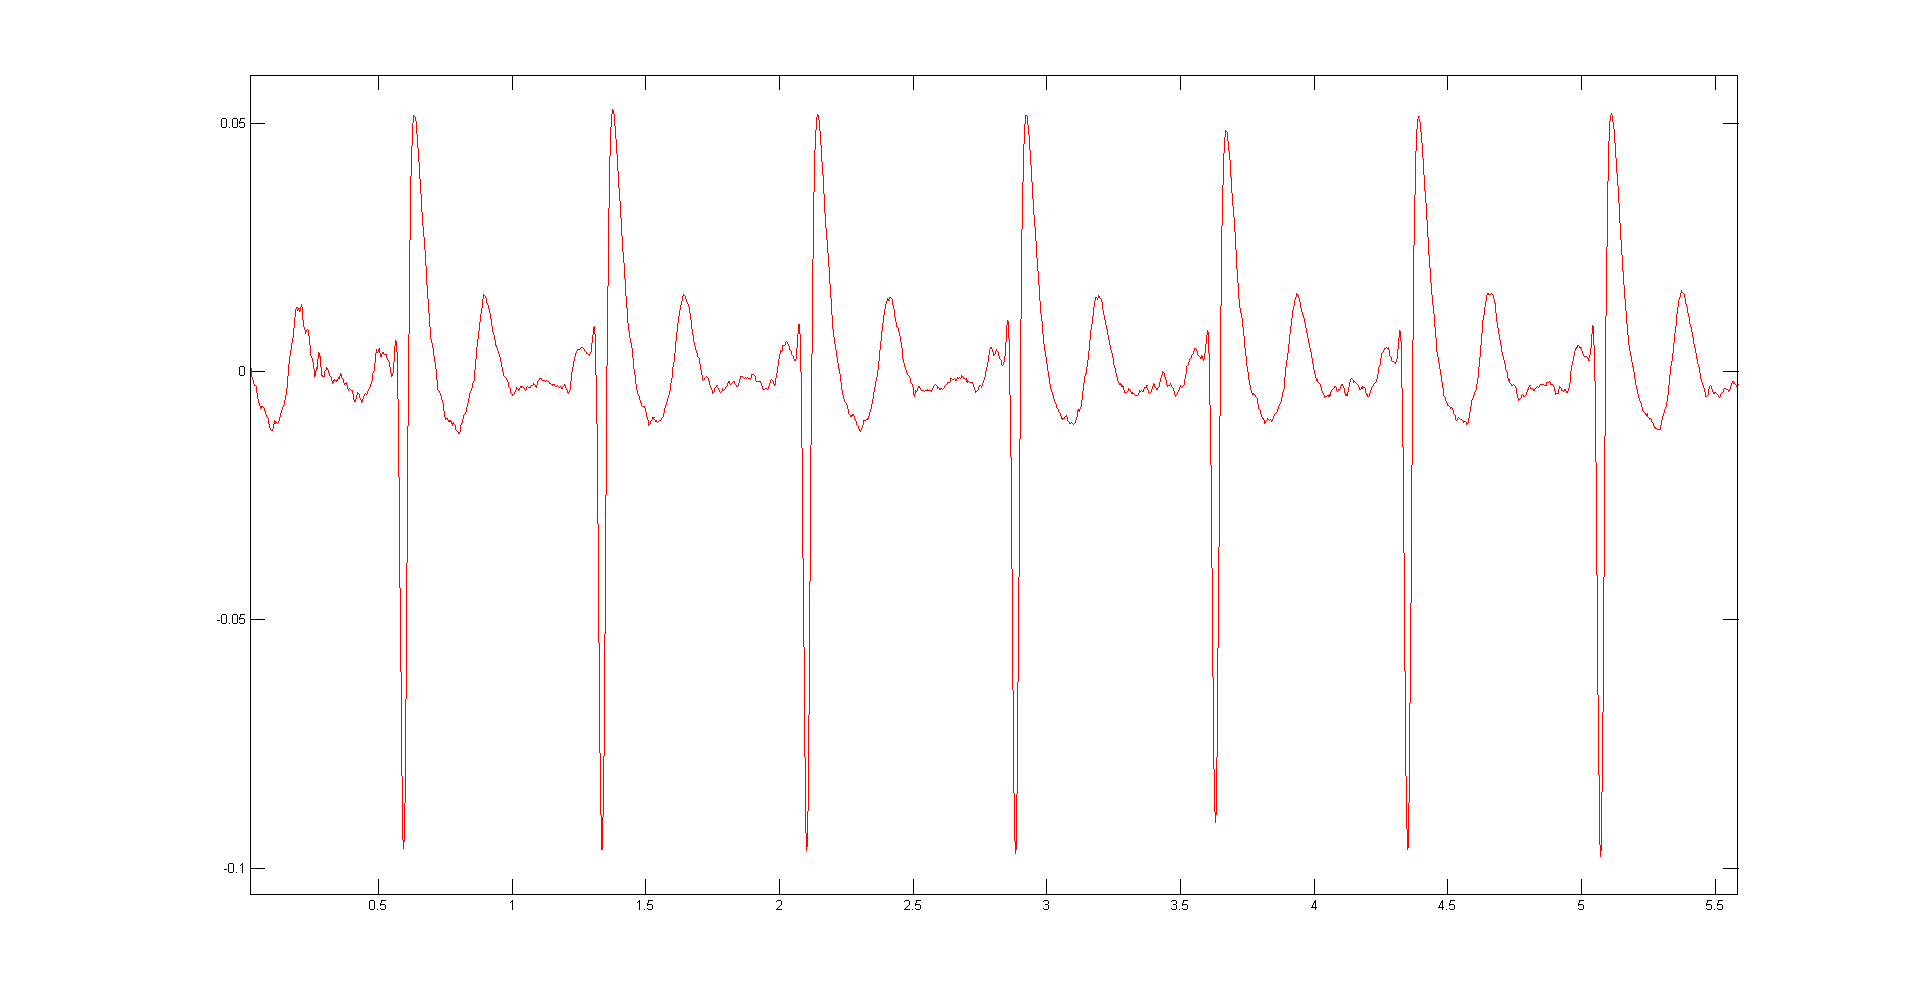
\includegraphics[scale=0.25]{../images/P2_FilteredECG} \\

\begin{lstlisting}
function H0 = notchFilter(N, lowFrequency, highFrequency)
    middle = N/2;
    lowK = 60 * lowFrequency;
    highK = 60 * highFrequency;
    H0 = ones(N,1);
    H0(middle-highK:middle-lowK) = 0;
    H0(middle+lowK:middle+highK) = 0;
end

N = length(xe0);
xe0fftUnshifted = fft(xe0)/N;
xe0fft = fftshift(xe0fftUnshifted);
H0 = notchFilter(N, 50, 70);
xe0Filtered = ifft(ifftshift(H0 .* xe0fft))*N;
\end{lstlisting}

\end{enumerate}

\end{document}